%%% CV de Romain REIGNIER créé grâce au template suivant :

%%% LaTeX Template: Designer's CV
%%%
%%% Source: http://www.howtotex.com/
%%% Feel free to distribute this template, but please keep the referal to HowToTeX.com.
%%% Date: March 2012

%%%%%%%%%%%%%%%%%%%%%%%%%%%%%%%%%%%%%
% Document properties and packages
%%%%%%%%%%%%%%%%%%%%%%%%%%%%%%%%%%%%%
\documentclass[a4paper,11pt,final]{memoir}

% misc
\renewcommand{\familydefault}{bch} % font
\pagestyle{empty}					         % no pagenumbering
\setlength{\parindent}{0pt}			   % no paragraph indentation

\usepackage[T1]{fontenc}
\usepackage[utf8]{inputenc}
% required packages (add your own)
\usepackage{flowfram}										 % column layout
\usepackage[top=1cm,left=1cm,right=1cm,bottom=1cm]{geometry}% margins
\usepackage{graphicx}										 % figures
\usepackage{url}											   % URLs
\usepackage[usenames,dvipsnames]{xcolor} % color
\usepackage{multicol}										 % columns env.
	\setlength{\multicolsep}{0pt}
\usepackage{paralist}										 % compact lists
\usepackage{tikz}
\usepackage{hyperref}
\hypersetup{colorlinks,citecolor=black,filecolor=black,linkcolor=black,urlcolor=black} % pour mettre les liens en noirs, sans cadre
\usepackage[francais]{babel}
\usepackage{microtype}

\definecolor{dark_gray}{rgb}{0.3,0.3,0.3}

%%%%%%%%%%%%%%%%%%%%%%%%%%%%%%%%%%%%%
% Create column layout
%%%%%%%%%%%%%%%%%%%%%%%%%%%%%%%%%%%%%
% define length commands
\setlength{\vcolumnsep}{\baselineskip}
\setlength{\columnsep}{\vcolumnsep}

% frame setup (flowfram package)
% left frame
\newflowframe{0.27\textwidth}{\textheight}{0pt}{0pt}[left]
	\newlength{\LeftMainSep}
	\setlength{\LeftMainSep}{0.26\textwidth}
	\addtolength{\LeftMainSep}{1\columnsep}

% small static frame for the vertical line
\newstaticframe{1.5pt}{\textheight}{\LeftMainSep}{0pt}

% content of the static frame
\begin{staticcontents}{1}
\hfill
\tikz{%
	\draw[loosely dotted,color=RoyalBlue,line width=1.5pt,yshift=0]
	(0,0) -- (0,\textheight);}%
\hfill\mbox{}
\end{staticcontents}

% right frame
\addtolength{\LeftMainSep}{1.5pt}
\addtolength{\LeftMainSep}{1\columnsep}
\newflowframe{0.68\textwidth}{\textheight}{\LeftMainSep}{0pt}[main01]

%%%%%%%%%%%%%%%%%%%%%%%%%%%%%%%%%%%%%
% define macros (for convience)
%%%%%%%%%%%%%%%%%%%%%%%%%%%%%%%%%%%%%
\newcommand{\Sep}{\vspace{1.5em}}
\newcommand{\SmallSep}{\vspace{0.5em}}

\newenvironment{AboutMe}
	{\ignorespaces}%\textbf{\color{RoyalBlue} About me}}
	{\SmallSep\ignorespacesafterend}

\newcommand{\CVSection}[1]
	{\Large\textbf{#1}\par
	\SmallSep\normalsize\normalfont}

\newcommand{\CVItem}[2]
	{\textbf{\color{RoyalBlue} #1 \color{dark_gray} #2}\normalsize\normalfont}

\newcommand{\city}[1]
	{{\small\color{dark_gray}\emph{#1}}\normalsize\normalfont}

\newcommand{\SkillSection}[1]
	{\normalsize{\textbf{#1\\}}\normalfont\small}%\footnotesize}

\newcommand{\SkillItem}[1]
	{\textbf{\color{RoyalBlue} #1}\normalfont\\}

%%%%%%%%%%%%%%%%%%%%%%%%%%%%%%%%%%%%%
% Begin document
%%%%%%%%%%%%%%%%%%%%%%%%%%%%%%%%%%%%%
\begin{document}

% Left frame
%%%%%%%%%%%%%%%%%%%%
% Photo
\begin{figure}
	\hfill
	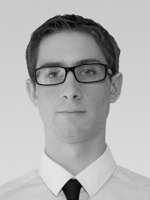
\includegraphics[width=0.5\columnwidth]{../IMG_7936-Modifier_cv}
	\vspace{-0.5cm}
\end{figure}

% Personnal Infos
\begin{flushright}\small
	%Romain \textsc{Reignier} \\
	117 rue de la République\\
	30290 Laudun l'Ardoise\\
	%France\\
	{\href{mailto:rom.reignier@gmail.com}{\nolinkurl{rom.reignier@gmail.com}}}\\
	06 09 52 16 18\\
	23 ans\\
	Permis B
\end{flushright}%\normalsize

\begin{flushleft}
% Languages
\SkillSection{Langues}
\SkillItem{Anglais}
Écrit et parlé (TOEIC : 920 pts)\\
\SkillItem{Espagnol}
Niveau Baccalauréat\\
\SkillItem{Allemand}
Notions
\SmallSep

% Engineering
\SkillSection{Compétences}
Conception mécanique\\
%Conception de systèmes\\
%Analyse des mécanismes\\
Résistance des matériaux\\
%Materials\\
Méthodes numériques\\
%Algorithmique\\
%Database\\
%Thermal transferts\\
Automatique\\
Systèmes asservis\\
Robotique\\
%Communication\\
%Vison par ordinateur\\
Traitement d'image
\SmallSep

% Computer Skills
\SkillSection{Informatique}
\SkillItem{CAO}
CATIA V5, SolidWorks, ADAMS\\
\SkillItem{Programmation}
\verb!C!/\verb!C++!, Python, Matlab/Simulink, LabView, Maple, OpenCV, Qt\\
\emph{Embarqué :} GNU/Linux, ROS, Arduino, AVR, dsPIC, ARM\\%, assembleur ST8\\
\SkillItem{Développement Web}
HTML5, CSS3, PHP, MySQL\\
\SkillItem{Bureautique}
Word, Excel (Visual Basic), PowerPoint, Access, Project, \LaTeX\\
\SkillItem{Graphisme}
Photoshop, Lightroom, Illustrator, Gimp, Inkscape, FinalCut Pro X\\
\SmallSep

% Sports
\SkillSection{Sports}
Cyclisme route \& VTT\\
Course à pied\\
%Swimming
\SmallSep

% Hobbies
\SkillSection{Loisirs}
Robotique\\
Mécanique\\
Machinisme Agricole\\
Agriculture\\
Photographie\\
Brevet d'Initiation à l'Aéronautique
\SmallSep

% Travels
\SkillSection{Voyages}
Malaisie, Singapour, Togo\\
InterRail 2014 : Amsterdam, Berlin, Prague, Vienne, Genève
%Pays-Bas, Allemagne, République Tchèque, Autriche, Suisse
\end{flushleft}
\framebreak

% Right frame
%%%%%%%%%%%%%%%%%%%%
%\Huge\bfseries {\color{RoyalBlue} Romain \textsc{Reignier}} \\
\Huge\bfseries {\color{RoyalBlue} Romain REIGNIER} \\
\Large\bfseries  Ingénieur Mécatronique et Robotique\\
% About me
%\begin{AboutMe}
%\end{AboutMe}

% Formation
\CVSection{Formation}

\CVItem{2012 -- 2015,}{SUPMÉCA} - \city{La Garde, PACA}\\
\emph{Institut Supérieur de Mécanique de Paris} (ex CESTI)\\
École d'ingénieurs généraliste à dominante mécanique, \\parcours \textbf{Robotique et Systèmes Mécatroniques}.
\SmallSep

\CVItem{2014 -- 2015,}{Université Sud Toulon Var} - \city{La Garde, PACA}\\
Master recherche Physique et Sciences de l'Ingénieur,\\ spécialité \textbf{Vision Commande}.
%Traitement d'image, vision par ordinateur, reconnaissance de formes, trajectographie, détection, estimation.
\SmallSep

\CVItem{2009 -- 2012,}{CPGE Victor Hugo} - \city{Caen, Normandie}\\
Classes Préparatoires aux concours d'entrée aux Grandes Écoles.\\
Physique et Sciences de l'Ingénieur (PSI).
%\SmallSep

%\CVItem{2006 -- 2009,}{Lycée Henri Cornat} - \city{Valognes, Normandie}\\
%Baccalauréat Scientique, spécialité Physique.
%With Honors.
\Sep
% Experience
\CVSection{Expériences}

\CVItem{Mars 2015 -- Août 2015,}{CEA} - \city{Marcoule, Languedoc-Roussillon}\\
Stage ingénieur.\\
Implémentation de ROS et du simulateur Gazebo sur un robot hexapode suivi d'un développement d'une nouvelle démarche pour le fanchissement de terrains irréguliers en vue d'une application dans le démantèlement.
\SmallSep

\CVItem{Septembre 2013 -- Janvier 2014,}{R\&D CLAAS Tractor} - \city{Vélizy, Île-de-France}\\
Stage assistant ingénieur.\\
Support à l'expert climatisation sur l'amélioration du système de ventilation de la cabine des tracteurs de fortes puissances.\\
Analyse des résultats de simulations et essais puis optimisation des conduits.
\SmallSep

\CVItem{Janvier 2013,}{DCNS} - \city{Cherbourg, Normandie}\\
Stage opérateur.\\
Travail sur des machines outils à commande numérique (tours, fraiseuses et alèseuses) pour la création de pièces de sécurité de sous-marins nucléaires.
\SmallSep

\CVItem{2006 -- 2012}{}\\
Emplois saisonniers : Deauville Polo Club, chantier de l'EPR pour EDF, tourneur-fraiseur, maintenance électroménager, ferme de polyculture-élevage.
\Sep

\CVSection{Projets \& Associations}
\CVItem{Projets de 3\ieme{} année}{}Étude conceptuelle d'un robot manipulateur mobile pour l'assainissement en milieu nucléaire en partenariat avec le CEA.\\
Instrumentation d'un aspirateur avec suivi de la consommation sur une application Android via Bluetooth Low Energy pour le laboratoire LISMMA.
\SmallSep

\CVItem{Projet de 2\ieme{} année}{}Restauration d'une chaîne d'automates programmables pneumatiques. Mécanique et programmation en Grafcet et Ladder.
\SmallSep

\CVItem{Club Robotique de Supméca}{}Conception, fabrication et programmation de robots pour la Coupe de France de robotique (Eurobot) 2013, 2014 et 2015.
\SmallSep

\CVItem{Supwave}{}Responsable de l'électronique embarquée sur un voilier autonome.
\SmallSep

\CVItem{Aérocorp}{}Responsable de l'électronique dans un avion d'aéromodélisme.
\SmallSep

\CVItem{Supméca Sans Frontières}{}Association humanitaire avec l'objectif d'assainir l'eau d'un orphelinat togolais. Gestion de projet, organisation d'évènements.
\SmallSep

\CVItem{Scouts et Guides de France}{}8 ans de scoutisme. Chef d'un camp de 30 enfants en 2012 et projet humanitaire d'un mois au Togo en août 2013.

%%%%%%%%%%%%%%%%%%%%%%%%%%%%%%%%%%%%%
% End document
%%%%%%%%%%%%%%%%%%%%%%%%%%%%%%%%%%%%%
\end{document}
